%  LaTeX support: latex@mdpi.com 
%  For support, please attach all files needed for compiling as well as the log file, and specify your operating system, LaTeX version, and LaTeX editor.

%=================================================================
\documentclass[journal,article,submit,pdftex,moreauthors]{Definitions/mdpi} 
%\documentclass[preprints,article,submit,pdftex,moreauthors]{Definitions/mdpi} 
% For posting an early version of this manuscript as a preprint, you may use "preprints" as the journal. Changing "submit" to "accept" before posting will remove line numbers.

%--------------------
% Class Options:
%--------------------
%----------
% journal
%----------
% Choose between the following MDPI journals:
% accountaudit, acoustics, actuators, addictions, adhesives, admsci, adolescents, aerobiology, aerospace, agriculture, agriengineering, agrochemicals, agronomy, ai, air, algorithms, allergies, alloys, amh, analytica, analytics, anatomia, anesthres, animals, antibiotics, antibodies, antioxidants, applbiosci, appliedchem, appliedmath, appliedphys, applmech, applmicrobiol, applnano, applsci, aquacj, architecture, arm, arthropoda, arts, asc, asi, astronomy, atmosphere, atoms, audiolres, automation, axioms, bacteria, batteries, bdcc, behavsci, beverages, biochem, bioengineering, biologics, biology, biomass, biomechanics, biomed, biomedicines, biomedinformatics, biomimetics, biomolecules, biophysica, biosensors, biosphere, biotech, birds, blockchains, bloods, blsf, brainsci, breath, buildings, businesses, cancers, carbon, cardiogenetics, catalysts, cells, ceramics, challenges, chemengineering, chemistry, chemosensors, chemproc, children, chips, cimb, civileng, cleantechnol, climate, clinbioenerg, clinpract, clockssleep, cmd, cmtr, coasts, coatings, colloids, colorants, commodities, complications, compounds, computation, computers, condensedmatter, conservation, constrmater, cosmetics, covid, crops, cryo, cryptography, crystals, csmf, ctn, curroncol, cyber, dairy, data, ddc, dentistry, dermato, dermatopathology, designs, devices, diabetology, diagnostics, dietetics, digital, disabilities, diseases, diversity, dna, drones, dynamics, earth, ebj, ecm, ecologies, econometrics, economies, education, eesp, ejihpe, electricity, electrochem, electronicmat, electronics, encyclopedia, endocrines, energies, eng, engproc, ent, entomology, entropy, environments, epidemiologia, epigenomes, esa, est, famsci, fermentation, fibers, fintech, fire, fishes, fluids, foods, forecasting, forensicsci, forests, fossstud, foundations, fractalfract, fuels, future, futureinternet, futureparasites, futurepharmacol, futurephys, futuretransp, galaxies, games, gases, gastroent, gastrointestdisord, gastronomy, gels, genealogy, genes, geographies, geohazards, geomatics, geometry, geosciences, geotechnics, geriatrics, glacies, grasses, greenhealth, gucdd, hardware, hazardousmatters, healthcare, hearts, hemato, hematolrep, heritage, higheredu, highthroughput, histories, horticulturae, hospitals, humanities, humans, hydrobiology, hydrogen, hydrology, hygiene, idr, iic, ijerph, ijfs, ijgi, ijmd, ijms, ijns, ijpb, ijt, ijtm, ijtpp, ime, immuno, informatics, information, infrastructures, inorganics, insects, instruments, inventions, iot, j, jal, jcdd, jcm, jcp, jcs, jcto, jdad, jdb, jeta, jfb, jfmk, jimaging, jintelligence, jlpea, jmahp, jmmp, jmms, jmp, jmse, jne, jnt, jof, joitmc, joma, jop, jor, journalmedia, jox, jpbi, jpm, jrfm, jsan, jtaer, jvd, jzbg, kidney, kidneydial, kinasesphosphatases, knowledge, labmed, laboratories, land, languages, laws, life, lights, limnolrev, lipidology, liquids, literature, livers, logics, logistics, lubricants, lymphatics, machines, macromol, magnetism, magnetochemistry, make, marinedrugs, materials, materproc, mathematics, mca, measurements, medicina, medicines, medsci, membranes, merits, metabolites, metals, meteorology, methane, metrics, metrology, micro, microarrays, microbiolres, microelectronics, micromachines, microorganisms, microplastics, microwave, minerals, mining, mmphys, modelling, molbank, molecules, mps, msf, mti, multimedia, muscles, nanoenergyadv, nanomanufacturing, nanomaterials, ncrna, ndt, network, neuroglia, neurolint, neurosci, nitrogen, notspecified, nursrep, nutraceuticals, nutrients, obesities, oceans, ohbm, onco, oncopathology, optics, oral, organics, organoids, osteology, oxygen, parasites, parasitologia, particles, pathogens, pathophysiology, pediatrrep, pets, pharmaceuticals, pharmaceutics, pharmacoepidemiology, pharmacy, philosophies, photochem, photonics, phycology, physchem, physics, physiologia, plants, plasma, platforms, pollutants, polymers, polysaccharides, populations, poultry, powders, preprints, proceedings, processes, prosthesis, proteomes, psf, psych, psychiatryint, psychoactives, psycholint, publications, purification, quantumrep, quaternary, qubs, radiation, reactions, realestate, receptors, recycling, regeneration, religions, remotesensing, reports, reprodmed, resources, rheumato, risks, robotics, rsee, ruminants, safety, sci, scipharm, sclerosis, seeds, sensors, separations, sexes, signals, sinusitis, siuj, skins, smartcities, sna, societies, socsci, software, soilsystems, solar, solids, spectroscj, sports, standards, stats, std, stresses, surfaces, surgeries, suschem, sustainability, symmetry, synbio, systems, tae, targets, taxonomy, technologies, telecom, test, textiles, thalassrep, therapeutics, thermo, timespace, tomography, tourismhosp, toxics, toxins, transplantology, transportation, traumacare, traumas, tropicalmed, universe, urbansci, uro, vaccines, vehicles, venereology, vetsci, vibration, virtualworlds, viruses, vision, waste, water, wem, wevj, wild, wind, women, world, youth, zoonoticdis

%---------
% article
%---------
% The default type of manuscript is "article", but can be replaced by: 
% abstract, addendum, article, benchmark, book, bookreview, briefcommunication, briefreport, casereport, changes, clinicopathologicalchallenge, comment, commentary, communication, conceptpaper, conferenceproceedings, correction, conferencereport, creative, datadescriptor, discussion, entry, expressionofconcern, extendedabstract, editorial, essay, erratum, fieldguide, hypothesis, interestingimages, letter, meetingreport, monograph, newbookreceived, obituary, opinion, proceedingpaper, projectreport, reply, retraction, review, perspective, protocol, shortnote, studyprotocol, supfile, systematicreview, technicalnote, viewpoint, guidelines, registeredreport, tutorial,  giantsinurology, urologyaroundtheworld
% supfile = supplementary materials

%----------
% submit
%----------
% The class option "submit" will be changed to "accept" by the Editorial Office when the paper is accepted. This will only make changes to the frontpage (e.g., the logo of the journal will get visible), the headings, and the copyright information. Also, line numbering will be removed. Journal info and pagination for accepted papers will also be assigned by the Editorial Office.

%------------------
% moreauthors
%------------------
% If there is only one author the class option oneauthor should be used. Otherwise use the class option moreauthors.

%---------
% pdftex
%---------
% The option pdftex is for use with pdfLaTeX. Remove "pdftex" for (1) compiling with LaTeX & dvi2pdf (if eps figures are used) or for (2) compiling with XeLaTeX.

%=================================================================
% MDPI internal commands - do not modify
\firstpage{1} 
\makeatletter 
\setcounter{page}{\@firstpage} 
\makeatother
\pubvolume{1}
\issuenum{1}
\articlenumber{0}
\pubyear{2025}
\copyrightyear{2025}
%\externaleditor{Firstname Lastname} % More than 1 editor, please add `` and '' before the last editor name
\datereceived{ } 
\daterevised{ } % Comment out if no revised date
\dateaccepted{ } 
\datepublished{ } 
%\datecorrected{} % For corrected papers: "Corrected: XXX" date in the original paper.
%\dateretracted{} % For retracted papers: "Retracted: XXX" date in the original paper.
\hreflink{https://doi.org/} % If needed use \linebreak
%\doinum{}
%\pdfoutput=1 % Uncommented for upload to arXiv.org
%\CorrStatement{yes}  % For updates
%\longauthorlist{yes} % For many authors that exceed the left citation part
%\IsAssociation{yes} % For association journals

%=================================================================
% Add packages and commands here. The following packages are loaded in our class file: fontenc, inputenc, calc, indentfirst, fancyhdr, graphicx, epstopdf, lastpage, ifthen, float, amsmath, amssymb, lineno, setspace, enumitem, mathpazo, booktabs, titlesec, etoolbox, tabto, xcolor, colortbl, soul, multirow, microtype, tikz, totcount, changepage, attrib, upgreek, array, tabularx, pbox, ragged2e, tocloft, marginnote, marginfix, enotez, amsthm, natbib, hyperref, cleveref, scrextend, url, geometry, newfloat, caption, draftwatermark, seqsplit
% cleveref: load \crefname definitions after \begin{document}

%=================================================================
% Please use the following mathematics environments: Theorem, Lemma, Corollary, Proposition, Characterization, Property, Problem, Example, ExamplesandDefinitions, Hypothesis, Remark, Definition, Notation, Assumption
%% For proofs, please use the proof environment (the amsthm package is loaded by the MDPI class).

%=================================================================
% Full title of the paper (Capitalized)
\Title{Title}

% MDPI internal command: Title for citation in the left column
\TitleCitation{Title}

% Author Orchid ID: enter ID or remove command
\newcommand{\orcidauthorA}{0000-0000-0000-000X} % Add \orcidA{} behind the author's name
%\newcommand{\orcidauthorB}{0000-0000-0000-000X} % Add \orcidB{} behind the author's name

% Authors, for the paper (add full first names)
\Author{Firstname Lastname $^{1}$\orcidA{}, Firstname Lastname $^{2}$ and Firstname Lastname $^{2,}$*}

%\longauthorlist{yes}

% MDPI internal command: Authors, for metadata in PDF
\AuthorNames{Firstname Lastname, Firstname Lastname and Firstname Lastname}

% Author citation:  
\AuthorCitation{Lastname, F.; Lastname, F.; Lastname, F.}

% Affiliations / Addresses (Add [1] after \address if there is only one affiliation.)
\address{%
$^{1}$ \quad Affiliation 1; e-mail@e-mail.com\\
$^{2}$ \quad Affiliation 2; e-mail@e-mail.com}

% Contact information of the corresponding author
\corres{Correspondence: e-mail@e-mail.com; Tel.: (optional; include country code; if there are multiple corresponding authors, add author initials) +xx-xxxx-xxx-xxxx (F.L.)}

% Current address and/or shared authorship
%\firstnote{Current address: Affiliation.}  
% Current address should not be the same as any items in the Affiliation section.

%\secondnote{These authors contributed equally to this work.}
% The commands \thirdnote{} till \eighthnote{} are available for further notes.

%\simplesumm{} % Simple summary

%\conference{} % An extended version of a conference paper

% Abstract (Do not insert blank lines, i.e. \\) 
\abstract{Hybrid satellite aerial terrestrial networks (HSATNs) are a promising solution towards tackling coverage and mobility issues in sixth generation (6G) networks.This paper presents a novel transmission scheme in the context of HSATNs,which allows pairs of terrestrial users to be simultaneously served via the satellite and the aerial base station (ABS).To this aim, non-orthogonal multiple access (NOMA) technique is adopted,at the ABS,by applying a rule-based hybrid NOMA and orthogonal multiple access (OMA) schemes.Comparisons between a standalone NOMA-based satellite transmission and the proposed method, reveal that significant sum-rate gains can be harvested under varying system parameters.}

% Keywords
\keyword{keyword 1; keyword 2; keyword 3 (List three to ten pertinent keywords specific to the article; yet reasonably common within the subject discipline.)} 

% The fields PACS, MSC, and JEL may be left empty or commented out if not applicable
%\PACS{J0101}
%\MSC{}
%\JEL{}

%%%%%%%%%%%%%%%%%%%%%%%%%%%%%%%%%%%%%%%%%%
% Only for the journal Diversity
%\LSID{\url{http://}}

%%%%%%%%%%%%%%%%%%%%%%%%%%%%%%%%%%%%%%%%%%
% Only for the journal Applied Sciences
%\featuredapplication{Authors are encouraged to provide a concise description of the specific application or a potential application of the work. This section is not mandatory.}
%%%%%%%%%%%%%%%%%%%%%%%%%%%%%%%%%%%%%%%%%%

%%%%%%%%%%%%%%%%%%%%%%%%%%%%%%%%%%%%%%%%%%
% Only for the journal Data
%\dataset{DOI number or link to the deposited data set if the data set is published separately. If the data set shall be published as a supplement to this paper, this field will be filled by the journal editors. In this case, please submit the data set as a supplement.}
%\datasetlicense{License under which the data set is made available (CC0, CC-BY, CC-BY-SA, CC-BY-NC, etc.)}

%%%%%%%%%%%%%%%%%%%%%%%%%%%%%%%%%%%%%%%%%%
% Only for the journal BioTech, Fishes, Neuroimaging and Toxins
%\keycontribution{The breakthroughs or highlights of the manuscript. Authors can write one or two sentences to describe the most important part of the paper.}

%%%%%%%%%%%%%%%%%%%%%%%%%%%%%%%%%%%%%%%%%%
% Only for the journal Encyclopedia
%\encyclopediadef{For entry manuscripts only: please provide a brief overview of the entry title instead of an abstract.}

%%%%%%%%%%%%%%%%%%%%%%%%%%%%%%%%%%%%%%%%%%
% Different journals have different requirements. Please check the specific journal guidelines in the "Instructions for Authors" on the journal's official website.
%\addhighlights{yes}
%\renewcommand{\addhighlights}{%
%
%\noindent The goal is to increase the discoverability and readability of the article via search engines and other scholars. Highlights should not be a copy of the abstract, but a simple text allowing the reader to quickly and simplified find out what the article is about and what can be cited from it. Each of these parts should be devoted up to 2~bullet points.\vspace{3pt}\\
%\textbf{What are the main findings?}
% \begin{itemize}[labelsep=2.5mm,topsep=-3pt]
% \item First bullet.
% \item Second bullet.
% \end{itemize}\vspace{3pt}
%\textbf{What is the implication of the main finding?}
% \begin{itemize}[labelsep=2.5mm,topsep=-3pt]
% \item First bullet.
% \item Second bullet.
% \end{itemize}
%}

%%%%%%%%%%%%%%%%%%%%%%%%%%%%%%%%%%%%%%%%%%
\begin{document}

%%%%%%%%%%%%%%%%%%%%%%%%%%%%%%%%%%%%%%%%%%
% The order of the section titles is different for some journals. Please refer to the "Instructions for Authors” on the journal homepage.

\section{Introduction}

The sixth generation (6G) network has already been commenced as a new research initiative, following on from the evolving 5G network.This new type of network envisions sophisticated device-to-device (D2D) and machine-to-machine (M2M) communications,innovative artificial intelligence (AI) techniques, Internet of Everything (IoE) applications connecting people, data, things through processes.Interoperability and convergence between terrestrial and satellite infrastructures will be a prerequisite in the 6G networking. Also, the new space era of non-terrestrial networks (NTNs) comprising of aerial networks, low Earth orbit (LEO) and especially very low Earth orbit (VLEO) satellites has emerged, enabling the path to 6G evolution.

Hybrid satellite-terrestrial networks (HSTNs) have been proposed as an efficient approach towards improving spectral efficiency and increasing the users’ reliability all over the world.The available spectrum resources of these networks can be further exploited by adopting the non-orthogonal multiple access (NOMA) principle.However, in the absence of line-of-sight (LoS) conditions, the performance of satellite communication systems is severely deteriorating.

In the context of HSTNs, the unmanned aerial vehicle (UAV)-based communications are expected to improve the performance in various ways.In general, the UAV-aided NOMA  schemes have gained the interest of the academia and the industry for various applications in the beyond 5G networks.Focusing on the scenario where the UAVs are adopted in satellite terrestrial communication networks, they could be employed in the NOMA scheme as an intermediate node for increasing the possibility of obtaining LoS conditions.

All-in-all, and to the best of our knowledge, no studies can be found related to the intelligent integration of aerial and satellite segments in 6G networks by utilizing a hybrid NOMA and orthogonal multiple access (OMA) transmission schemes. Motivated by this observation, in this paper, we propose a novel satellite aerial terrestrial cooperative network scheme, which will be termed SATCON. More specifically, SATCON is formed with the integration of aerial base station (ABS) in the existing satellite network by efficiently combining two unsupervised machine learning (ML) algorithms, namely k-means and k-medoids. Furthermore, the proposed system promotes efficient cooperation between ABS and satellite through an innovative hybrid NOMA/OMA approach, avoiding the waste of resources and energy.Compared to standalone satellite NOMA transmission with optimal user pairing, namely SAT-NOMA, SATCON increases the sum rate and, at the same time, provides higher spectral efficiency for varying satellite channel conditions and ABS bandwidth.
%%%%%%%%%%%%%%%%%%%%%%%%%%%%%%%%%%%%%%%%%%
\section{Materials and Methods}

\subsection{UAV-Assisted Downlink Transmission}
As shown in Figure~\ref{fig:system_model}, the considered SAGIN consists of $\mathbf{U}$ UAVs denoted by $\mathcal{U} = {1, 2, \dots, U}$ and $\mathbf{S}$ LEO satellites indicated by $\mathcal{S} = {1, 2, \dots, S}$. In addition, $\mathbf{K}$ IoT devices randomly scattered on the ground are represented as $\mathcal{K} = {1, 2, \dots, K}$.

In the considered downlink architecture, Internet-of-Things (IoT) devices may either receive data directly from a low Earth orbit (LEO) satellite or be served via an unmanned aerial vehicle (UAV) acting as a decode-and-forward relay. In the latter case, the UAV receives and decodes the satellite downlink signals over the satellite-to-air (S2A) link and forwards the decoded information to ground devices through the air-to-ground (A2G) link.

Power-domain NOMA multiplexes multiple users on the same time–frequency resource block via superposition coding with different power allocation coefficients.
Within this framework, the satellite performs NOMA user pairing based on the satellite–user channel conditions and transmits power-domain superimposed downlink signals to each paired user group. Since the unmanned aerial vehicle (UAV) is located within the satellite coverage area, it can also receive and decode the same superimposed signals via the satellite-to-air (S2A) link. In this context, whether the UAV can effectively enhance the downlink performance depends on the transmission capability of its forwarding link. Therefore, the potential benefit of UAV-assisted transmission is determined by the quality of the air-to-ground (A2G) links between the UAV and the ground users.

Accordingly, the UAV evaluates whether auxiliary relaying should be activated and selects the appropriate transmission mode, i.e., NOMA or orthogonal multiple access (OMA), based on the A2G channel conditions. UAV-assisted transmission is enabled only when the achievable downlink rate via the UAV exceeds that of the direct satellite link. Specifically, if a considered user pair can achieve higher downlink rates under the UAV-side NOMA pairing policy, the UAV adopts NOMA transmission to serve this pair. Otherwise, if only a single user benefits from UAV relaying, the UAV selectively serves this user using OMA transmission, while the remaining users continue to be served directly by the satellite.

% Figure 1
\begin{figure}[!htbp]
\centering
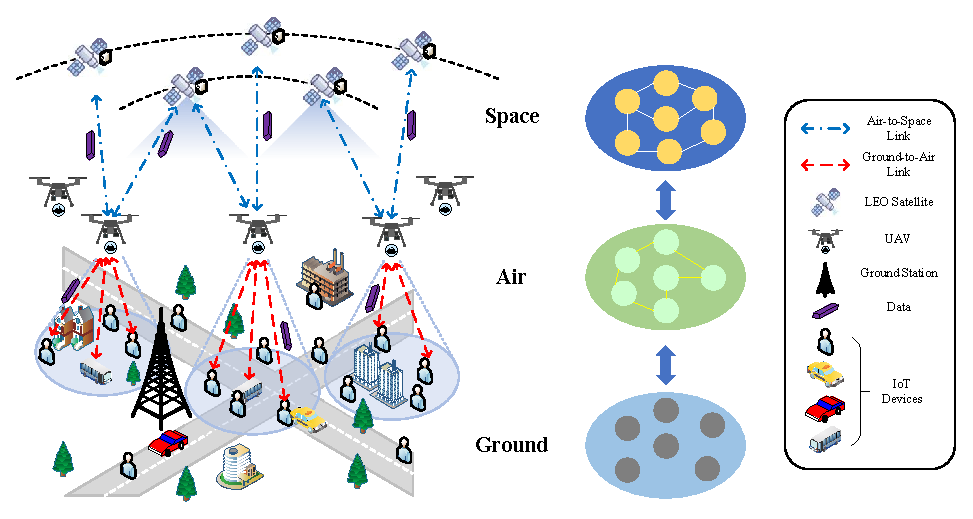
\includegraphics[width=0.95\columnwidth]{Definitions/figure1}
\caption{Illustration of the uplink communication procedure in SAGIN, where UAVs act as aerial aggregators to collect data from spatially distributed IoT devices and subsequently offload the aggregated data to LEO satellites.}
\label{fig:system_model}
\end{figure}

\subsection{Downlink Transmission Channel Quality Indicator}
The satellite performs downlink NOMA user pairing based on the channel quality of the satellite-to-ground (S2G) links. 
In contrast, the ABS decides whether to participate in decode-and-forward relaying and determines the corresponding transmission mode (NOMA or OMA) mainly according to the air-to-ground (A2G) channel conditions.

Specifically, the S2G and A2G links are characterized by the channel quality indicator $\Gamma$, which incorporates small-scale fading effects and is mainly used for user ordering and decision making. 

For the satellite transmission, the land mobile satellite (LMS) channel between the satellite and ground IoT $k$ $(1 \leq k \leq 2K)$ is characterized by the complex channel coefficient $h_k^s$, which captures the small-scale fading effects. Accordingly, the corresponding normalized satellite downlink channel quality indicator (CQI) is defined as
\begin{equation}
\Gamma_k^s = \frac{G_t^s G_r^s}{L_k^{\mathrm{FS}} N_s} |h_k^s|^2 ,
\label{normalized indicator}
\end{equation}
where $G_t^s$ and $G_r^s$ denote the satellite transmit and user receive antenna gains, respectively, $L_k^{\mathrm{FS}}$ represents the free-space path loss of the satellite-to-ground link for user $k$, $N_s$ is the noise power at the ground user receiver, and $|h_k^s|^2$ denotes the instantaneous power gain of the LMS channel.

Based on the defined CQI, the satellite performs NOMA user ordering and pairing to enable power-domain multiplexing. Specifically, the IoTs are first sorted in ascending order according to their CQI values
\begin{equation}
\Gamma_1^s \le \Gamma_2^s \le \cdots \le \Gamma_{2K}^s .
\end{equation}

Following the optimal NOMA user pairing strategy in \cite{zhu2018optimal}, this pairing strategy exploits the CQI disparity among users to enhance spectral efficiency while maintaining fairness in NOMA transmission.
The satellite pairs the $k$-th weakest user with the $(2K-k+1)$-th strongest user. 
As a result, each NOMA pair consists of a weak satellite-channel user and a strong satellite-channel user, denoted by $\mathrm{IoT}_i^s$ and $\mathrm{IoT}_j^s$, respectively, satisfying $\Gamma_j^s \ge \Gamma_i^s$.
We adopt the standard power-domain NOMA model with superposition coding at the transmitter and successive interference cancellation (SIC) at the receivers. 
Since SIC is not the focus of this work, ideal SIC is assumed and the corresponding achievable rates  and power allocation coefficients follow the conventional NOMA expressions.

For the ABS-assisted transmission, the air-to-ground (A2G) channel between the ABS and ground user $k$ $(1 \leq k \leq K)$ is characterized by the complex channel coefficient $h_k^d$, which captures the small-scale fading effects of the A2G link. 
By incorporating the ABS and user antenna gains, the A2G path loss dependent on the ABS altitude $h$ and the horizontal distance $r_k$, as well as the receiver noise power, the corresponding normalized A2G CQI is defined as
\begin{equation}
\Gamma_k^d = \frac{G_t^d G_r^d}{L_k^{\mathrm{A2G}}(h, r_k) N_d} |h_k^d|^2 .
\end{equation}
where $G_t^d$ and $G_r^d$ denote the ABS transmit and user receive antenna gains, respectively, $L_k^{\mathrm{A2G}}(h, r_k)$ represents the A2G path loss as a function of the ABS altitude $h$ and the horizontal distance $r_k$, $N_d$ is the receiver noise power associated with the A2G link, and $|h_k^d|^2$ denotes the instantaneous power gain.

The defined A2G CQI will be subsequently used by the ABS to evaluate the potential performance gain of relay-assisted transmission by characterizing the quality of the air-to-ground link. Specifically, a higher A2G CQI indicates more favorable access conditions between the ABS and the ground users, making relay-assisted transmission more likely to outperform direct satellite transmission and thus influencing the selection of the corresponding transmission mode.

\subsection{Downlink Transmission Constraints and Bottlenecks}
Before forwarding the satellite signals to the ground users, the ABS must successfully receive and decode the superimposed downlink signals over the satellite-to-air (S2A) backhaul link. As a result, the S2A link imposes a fundamental constraint on the achievable performance of ABS-assisted transmission and constitutes a key bottleneck in the downlink.

To characterize this bottleneck, the quality of the S2A link is described by the following normalized backhaul channel parameter
\begin{equation}
\Lambda_{sd} = \frac{G_t^s G_r^{sd}}{L_{sd}^{\mathrm{FS}} N_{sd}} ,
\end{equation}
where $G_t^s$ and $G_r^{sd}$ denote the satellite transmit and ABS receive antenna gains, respectively, $L_{sd}^{\mathrm{FS}}$ represents the free-space path loss of the S2A link, and $N_{sd}$ is the receiver noise power at the ABS.

It is worth noting that, regardless of the quality of the air-to-ground (A2G) access links, the end-to-end downlink rate achievable via ABS-assisted transmission is upper-bounded by the decoding capability of the S2A backhaul link. Consequently, the S2A link acts as a bottleneck that limits the effectiveness of relay-assisted downlink transmission.

The above modeling framework establishes the downlink transmission modes, channel quality indicators, and fundamental bottlenecks of the considered satellite–ABS–ground system, which together provide the basis for the subsequent algorithmic design and optimization.

It is worth noting that, although the S2A backhaul link constitutes a fundamental bottleneck for ABS-assisted downlink transmission, it is not directly optimized as an independent design variable. Instead, the proposed three-step framework implicitly accounts for this constraint through the joint design of transmission mode selection, S2A resource allocation, and ABS deployment. Specifically, inefficient relay-assisted transmission modes are avoided during the mode selection stage, the decode-and-forward bottleneck is eliminated through appropriate S2A resource allocation, and the impact of the backhaul constraint is further alleviated via ABS position optimization, thereby effectively mitigating the influence of the S2A bottleneck on system performance.

\section{Algorithm Design and Implementation}

\subsection{Transmission Mode Selection}
Although each user may theoretically receive downlink signals from both the satellite and the ABS,the transmission mode is determined at the ABS prior to downlink forwarding.
This is because simultaneous transmission of multiple NOMA signals would result in unmanageable inter-layer interference and excessive backhaul and power consumption. Therefore, the ABS determines in advance whether and how to forward the satellite signals, ensuring that only beneficial transmissions are activated.

When ABS-OMA is selected for a user, the satellite continues its NOMA broadcast as the baseline transmission, while the ABS selectively forwards the decoded signal only to the intended user using OMA. The paired user is served exclusively by the satellite in that time slot.

Although ABS-OMA may result in a lower sum rate for the corresponding user pair within the same transmission interval compared to ABS-NOMA, it guarantees that the user served by the ABS achieves a higher rate than direct satellite transmission, while avoiding unnecessary forwarding for the other user.

In general, under a downlink transmission where the available bandwidth $B$ is shared by $K$ user pairs, the achievable rate of user $k$ can be expressed in a system-level form as
\begin{equation}
R_k = \frac{B}{K}\log_2\!\left(1+\mathrm{SINR}_k\right),
\label{eq:unified_rate}
\end{equation}
where $\mathrm{SINR}_k$ captures the effect of power allocation and multi-user interference under the adopted transmission scheme.

After satellite NOMA pairing based on the CQI $\Gamma_k^{s}$,the downlink rate of user $k$ under satellite transmission follows the expression in~\eqref{eq:unified_rate}.
Accordingly, the satellite downlink rate is denoted by $R_k^{s}$.
For each satellite NOMA pair $(i,j)$ with $\Gamma_i^{s}\le \Gamma_j^{s}$, let $\beta_j^{s}\in(0,1)$ denote the power allocation factor for the strong user.
The corresponding SINRs are given by
\begin{align}
\mathrm{SINR}^{s}_{i}
&=\frac{(1-\beta_j^{s})P_s\,\Gamma_i^{s}}{\beta_j^{s}P_s\,\Gamma_i^{s}+1},
\label{eq:sat_sinr_weak}\\
\mathrm{SINR}^{s}_{j}
&=\beta_j^{s}P_s\,\Gamma_j^{s},
\label{eq:sat_sinr_strong}
\end{align}
where the strong user applies standard SIC to remove the weak user's signal prior to decoding its own message.

Similarly, for ABS transmission, the achievable access link rate of user $k$, denoted by $R_k^{d}$, follows the same rate expression in~\eqref{eq:unified_rate}, with the ABS bandwidth $B_d$ and the corresponding $\mathrm{SINR}_k^{d}$ determined by the A2G channel conditions.

Unlike satellite transmission, ABS forwarding is additionally constrained by the satellite-to-air (S2A) backhaul link. 
As a result, the effective downlink rates provided by the ABS under NOMA and OMA modes are given by
\begin{equation}
R_k^{dn} = \min\!\left(R_k^{d},\, R_k^{sd}\right), \qquad
R_k^{do} = \min\!\left(R_k^{o},\, R_k^{sd}\right),
\label{eq:abs_backhaul_constraint}
\end{equation}
where $R_k^{sd}$ denotes the maximum decodable rate at the ABS over the S2A link.

From an optimization perspective, the greedy transmission mode selector aims to maximize the aggregate achievable rate of each ABS-formed user pair within the same transmission interval. Accordingly, the transmission mode is selected by comparing the pair-wise sum rates under all feasible modes.


For each ABS-formed user pair $(u,v)$, the ABS determines the transmission mode by comparing the achievable rates under different forwarding options
\begin{equation}
m^{\star} = \arg\max_{m \in \mathcal{M}}
\left( R_u^{(m)} + R_v^{(m)} \right),
\end{equation}
where $\mathcal{M}=\{\text{SAT},\text{ABS-NOMA},\text{ABS-OMA-}u,\text{ABS-OMA-}v\}$ denotes the set of feasible transmission modes, and $R_u^{(m)}$ and $R_v^{(m)}$ represent the achievable downlink rates of users $u$ and $v$, respectively, under transmission mode $m$.


Accordingly, the following four cases are considered
\begin{itemize}
    \item \textbf{Case~1: ABS-assisted NOMA transmission.}  
    If $R_u^{dn} > R_u^{s}$ and $R_v^{dn} > R_v^{s}$,
    the ABS serves the user pair using NOMA. In this case, both users are
    forwarded by the ABS and achieve rates $R_u^{dn}$ and $R_v^{dn}$,
    respectively.

    \item \textbf{Case~2: ABS-assisted OMA transmission for user $u$.}  
    If $R_u^{do} > R_u^{s}$ while $R_v^{dn} \le R_v^{s}$,
    the ABS utilizes OMA and transmits only to user $u$ during the time slot
    allocated to this pair. User $u$ achieves a rate of $R_u^{do}$, whereas
    user $v$ is served directly by the satellite.

    \item \textbf{Case~3: ABS-assisted OMA transmission for user $v$.}  
    If $R_v^{do} > R_v^{s}$ while $R_u^{dn} \le R_u^{s}$,
    the ABS serves only user $v$ using OMA, and user $u$ is served by the
    satellite.

    \item \textbf{Case~4: Satellite-only transmission.}  
    Otherwise, ABS forwarding is not profitable for this user pair.
    Hence, the ABS remains silent and both users are served directly by
    the satellite in order to avoid unnecessary resource consumption.
\end{itemize}

It is worth emphasizing that the transmission mode selection is inherently performed at the level of ABS-formed user pairs.This is because a single ABS transmission action—whether employing NOMA, OMA, or remaining silent—is physically defined only with respect to the specific pair of users that the ABS simultaneously serves within a given transmission interval.As a result, the feasibility, decoding order, and achievable rates of an ABS transmission cannot be meaningfully evaluated outside the context of the corresponding ABS-formed pair.

Moreover, the role of the ABS in the framework is to enhance,rather than replace, the baseline satellite downlink. 
Accordingly, ABS forwarding is activated only when it can provide tangible rate improvements for the assisted users without compromising the overall downlink efficiency.
Otherwise, the ABS remains silent to avoid unnecessary backhaul usage and transmission overhead.

The proposed greedy selector operates independently on each ABS-formed user pair, leading to a linear computational complexity with respect to the number of pairs. 
In contrast, an exhaustive search over all possible mode combinations incurs an exponential complexity and becomes infeasible even for a moderate number of user pairs. 
Therefore, the greedy strategy offers an attractive trade-off between performance and computational efficiency, making it suitable for practical implementations.

\subsection{Resource allocation}

After determining the transmission mode for all users, the S2A backhaul bandwidth is allocated to those users relying on the ABS-assisted relaying.
Although users may be re-paired at the ABS side to facilitate access transmission, the S2A bandwidth allocation remains satellite-pair based, since the S2A link carries pre-formed satellite NOMA superimposed signals.

For any user utilizing ABS services, the achievable end-to-end downlink rate is constrained by
\begin{equation}
R_{u}^{\mathrm{E2E}} = \min\!\left( R_{u}^{\mathrm{A2G}},\, R_{u}^{\mathrm{S2A}} \right),
\end{equation}
where $R_{u}^{\mathrm{A2G}}$ denotes the achievable access-link rate, and
$R_{u}^{\mathrm{S2A}}$ denotes the achievable decoding rate of user $u$ at the ABS over the S2A backhaul link.
As a consequence, allocating excessive S2A bandwidth yields no further throughput gain once the S2A decoding rate exceeds the corresponding A2G rate, whereas insufficient S2A bandwidth directly degrades the achievable end-to-end performance.

Therefore, the objective of S2A resource allocation is not to maximize the S2A rate itself, but to allocate just enough backhaul bandwidth to eliminate the decode-and-forward (DF) bottleneck, while respecting the total satellite bandwidth constraint.
Under this design, the end-to-end rate of each user forwarded by the ABS is no longer limited by the S2A link, but is instead entirely determined by the A2G transmission capability.

Under satellite NOMA transmission, the achievable S2A decoding rate of each user at the ABS depends on the allocated S2A bandwidth and the effective signal-to-interference-plus-noise ratio (SINR) experienced during decoding.
Specifically, for the $k$-th satellite-side user pair, the S2A decoding rates of the strong and weak users can be expressed as
\begin{align}
R_{k,j}^{\mathrm{S2A}} &= b_k \log_2\!\left(1 + \beta_{k,j} \gamma_s h_{s2a}\right), \\
R_{k,i}^{\mathrm{S2A}} &= b_k \log_2\!\left(1 + 
\frac{\beta_{k,i} \gamma_s h_{s2a}}
{1 + \beta_{k,j} \gamma_s h_{s2a}}
\right),
\end{align}
where $b_k$ denotes the S2A bandwidth allocated to the $k$-th satellite-side user pair, $\gamma_s$ represents the average satellite SNR, and $h_{s2a}$ denotes the large-scale channel gain of the S2A link between the satellite and the ABS.
The parameters $\beta_{k,j}$ and $\beta_{k,i}$ are the satellite-side power allocation coefficients associated with the strong and weak users, respectively, which are determined by the satellite NOMA transmission strategy and remain fixed during the resource allocation process.
The above expressions are introduced to characterize the decoding feasibility at the ABS and to establish a monotonic relationship between the allocated S2A bandwidth and the achievable decoding rate, rather than to perform physical-layer optimization.

Accordingly, the allocated S2A bandwidth should satisfy the following decoding constraint
\begin{equation}
R_{k,u}^{\mathrm{S2A}}(b_k) \ge R_{k,u}^{\mathrm{A2G}}, \quad u \in \{i,j\}.
\end{equation}

Since the S2A decoding rate is a monotonically increasing function of the allocated bandwidth,
the minimum S2A bandwidth required to satisfy the DF decoding constraint for user $u$
can be obtained by directly inverting the inequality as
\begin{equation}
b_{k,u}^{\min}
=
\frac{R_{k,u}^{\mathrm{A2G}}}
{\log_2\!\left(1+\gamma_{k,u}^{\mathrm{eff}}\right)} .
\end{equation}

Under satellite NOMA transmission, both users in the $k$-th satellite-side pair must be successfully decoded at the ABS.
Therefore, the minimum bandwidth required for the $k$-th pair is determined by the most stringent decoding constraint
\begin{equation}
b_k^{\min}
=
\max \!\left( b_{k,i}^{\min},\, b_{k,j}^{\min} \right).
\end{equation}

Given the total satellite bandwidth constraint
\begin{equation}
\sum_{k=1}^{K} b_k^{\min} \le B_s ,
\end{equation}
the S2A bandwidth allocation problem aims to determine $\{b_k\}$ such that the DF decoding constraints are satisfied for all users.
This problem is convex and can be efficiently solved using the Karush--Kuhn--Tucker (KKT) conditions.

In some cases, the aggregate minimum S2A bandwidth demand may exceed the available satellite bandwidth, i.e.,
\begin{equation}
\sum_{k=1}^{K} b_k^{\min} > B_s .
\end{equation}
To guarantee feasibility under the limited satellite bandwidth, a proportional scaling strategy is applied.
Specifically, all S2A bandwidth allocations are uniformly scaled as
\begin{equation}
b_k = b_k^{\min} \cdot \frac{B_s}{\sum_{k=1}^{K} b_k^{\min}}, \quad \forall k .
\end{equation}

The proportional scaling preserves the relative bandwidth demands among different satellite-side user pairs, thereby avoiding abrupt structural changes in the transmission configuration.
Although this operation may prevent the S2A decoding rate from fully matching the corresponding A2G rate for all users, it ensures a feasible and stable bandwidth allocation without introducing additional combinatorial optimization.

It is worth noting that, when the satellite bandwidth is insufficient to support all A2G demands, the achievable end-to-end rates may be lower than the ideal values predicted by the greedy mode selection.
This is because the greedy mode selection is performed under the assumption that the S2A backhaul is not the limiting factor, and thus identifies the transmission structure that maximizes the potential system throughput.
The subsequent bandwidth scaling reflects the physical limitation of the satellite backhaul rather than a suboptimal design choice.
By separating the structural decision from the feasibility enforcement, the proposed framework achieves a favorable balance between performance, computational tractability, and algorithmic stability.


\subsection{ABS Position Optimisation}
The ABS position optimisation is formulated as a bound-constrained continuous optimisation problem, where the objective function is evaluated through a complete re-execution of the proposed greedy mode selection and KKT-based resource allocation, thus enabling true end-to-end performance-driven placement.

In the proposed framework, the position of the aerial base station (ABS) plays a critical role in shaping both the access and backhaul link qualities, and consequently affects transmission mode selection and resource allocation. 
Unlike conventional geometry-driven placement strategies, the ABS location is optimized here in a communication-performance-driven manner, jointly accounting for the air-to-ground (A2G) access links, the satellite-to-air (S2A) backhaul, and the resulting end-to-end achievable rates.

Specifically, we formulate the ABS placement as a bound-constrained continuous optimization problem, where the three-dimensional ABS position is denoted by
\begin{equation}
\mathbf{p}_d = (x_d, y_d, h_d),
\end{equation}
with $(x_d, y_d)$ representing the horizontal coordinates and $h_d$ denoting the flight altitude. The optimization objective is to maximize the system sum rate after transmission mode selection and resource allocation, which can be expressed as
\begin{equation}
\max_{\mathbf{p}_d} \; \sum_{u \in \mathcal{U}} R_u(\mathbf{p}_d),
\end{equation}
subject to the following feasibility constraints
\begin{align}
- R_{\mathrm{cov}} \leq x_d \leq R_{\mathrm{cov}}, \\
- R_{\mathrm{cov}} \leq y_d \leq R_{\mathrm{cov}}, \\
h_{\min} \leq h_d \leq h_{\max},
\end{align}
where $R_{\mathrm{cov}}$ denotes the horizontal coverage radius of the ABS, and $[h_{\min}, h_{\max}]$ specifies the allowable altitude range.

It is important to note that the objective function in~(XX) does not admit a closed-form expression. For a given ABS position $\mathbf{p}_d$, the achievable rate $R_u(\mathbf{p}_d)$ of each user depends on multiple interrelated components, including the A2G channel gains, the S2A backhaul quality, the ABS-based user pairing, the greedy transmission mode selection, and the KKT-based S2A bandwidth allocation. As a result, each evaluation of the objective function requires a complete execution of the proposed greedy mode selector and the KKT resource allocator, thereby capturing the true end-to-end system performance.

Due to the continuous nature of the optimization variables and the presence of non-smooth operations such as mode switching and minimum-rate constraints imposed by decode-and-forward relaying, the resulting problem is inherently non-convex. To efficiently solve this problem under practical boundary constraints, we adopt the limited-memory Broyden--Fletcher--Goldfarb--Shanno algorithm with box constraints (L-BFGS-B). This method is well suited for large-scale bound-constrained optimization and enables efficient convergence using numerical gradient approximations without requiring explicit gradient expressions.

The optimization procedure is initialized at the geometric centroid of the user distribution in the horizontal plane, combined with a nominal altitude within the feasible range. To ensure numerical stability and reproducibility during the iterative optimization, the small-scale fading realizations of the A2G channels are fixed throughout the process, such that the objective function remains deterministic. At each iteration, the ABS position is updated according to the L-BFGS-B search direction, and the resulting candidate solution is projected onto the feasible domain defined by the coverage and altitude constraints.

By directly optimizing the communication performance rather than geometric proximity, the proposed ABS placement strategy effectively captures the coupled impact of position, transmission mode selection, and resource allocation. This joint optimization mechanism enables the ABS to dynamically balance A2G access quality and S2A backhaul capacity, thereby improving the overall system throughput.

%%%%%%%%%%%%%%%%%%%%%%%%%%%%%%%%%%%%%%%%%%
\section{Results}

The proposed SATCON framework was implemented in Python, and all simulations were conducted on a workstation equipped with an Intel Core i7 processor and 16~GB RAM. Unless otherwise specified, the simulation parameters are summarized in Table~\ref{tab:sim_params}.
\begin{table}[t]
\centering
\caption{Simulation Parameters}
\label{tab:sim_params}
\begin{tabular}{lll}
\toprule
\textbf{Parameter} & \textbf{Symbol} & \textbf{Value} \\
\midrule
Number of users & $N$ & 32 \\
Coverage radius & $R$ & 500 m \\
Satellite altitude & $H_s$ & 600 km \\
Satellite elevation angle & $E$ & $10^\circ$, $20^\circ$, $40^\circ$ \\
Satellite bandwidth & $B_s$ & 10 MHz \\
ABS bandwidth & $B_d$ & 0.4, 1.2, 2.0, 3.0 MHz \\
Satellite transmit power & $P_s$ & 30 dBm \\
ABS transmit power & $P_d$ & 23 dBm \\
Satellite antenna gain & $G_s^t$ & 40 dBi \\
ABS antenna gain & $G_d^t$ & 5 dBi \\
User antenna gain & $G_u^r$ & 0 dBi \\
ABS altitude range & $h_d$ & 100--500 m \\
Carrier frequency (S2G) & $f_s$ & 2 GHz \\
Carrier frequency (A2G) & $f_d$ & 2.4 GHz \\
Noise power density & $N_0$ & $-174$ dBm/Hz \\
Path loss exponent (A2G) & $\alpha$ & 2.5 \\
Random seed & -- & 42 \\
\bottomrule
\end{tabular}
\end{table}

We consider a single-beam satellite coverage scenario, where $N$ ground users are uniformly distributed within a circular service area of radius $R=500$~m. A low Earth orbit (LEO) satellite at altitude $H_s=600$~km provides downlink transmission to the users either directly or via an aerial base station (ABS) acting as a decode-and-forward relay. The ABS altitude is constrained within the range $h_d \in [100, 500]$~m.

For the satellite-to-ground (S2G) and satellite-to-ABS (S2A) links, large-scale path loss is determined by satellite geometry and elevation angle $E$, while small-scale fading is neglected due to the dominant line-of-sight (LoS) component. For the air-to-ground (A2G) links, we adopt a distance-dependent path loss model with exponent $\alpha=2.5$ and incorporate Rayleigh fading to capture small-scale channel variations.

To ensure statistical reliability, each simulation result is obtained by averaging over 50 independent Monte Carlo realizations with different user locations and fading samples, while fixing the random seed for reproducibility. Noise power is computed based on a noise power spectral density of $N_0=-174$~dBm/Hz.

We evaluate system performance using the following metrics
\begin{itemize}
  \item \emph{System sum rate (Mbps)}: defined as the aggregate downlink throughput of all users in the network.
  \item \emph{Spectral efficiency (bps/Hz)}: computed as the system sum rate normalized by the total satellite bandwidth.
  \item \emph{Average user rate (Mbps)}: obtained by dividing the system sum rate by the number of served users.
\end{itemize}
These metrics jointly reflect the efficiency, scalability, and fairness of the proposed framework.Unless otherwise specified, these metrics are reported as the average values over all Monte Carlo realizations.

\subsection{Overall Performance Comparison with Baseline Schemes}

This subsection evaluates the overall performance of the proposed SATCON framework by comparing it with representative baseline schemes under identical system settings. All schemes share the same satellite bandwidth, transmit power, user distribution, and channel models, ensuring a fair and meaningful comparison.

Specifically, the following baseline schemes are considered:
\begin{itemize}
  \item \emph{SAT-NOMA}: a conventional satellite-only transmission scheme where all users are directly served by the satellite using NOMA, without ABS assistance.
  \item \emph{Heuristic + Uniform}: a sub-optimal scheme that employs heuristic transmission mode selection, uniform bandwidth allocation, and fixed ABS placement based on geometric considerations.
  \item \emph{Heuristic + Uniform + k-means} (Baseline): a complete baseline framework that integrates heuristic mode selection, uniform resource allocation, and ABS placement via k-means clustering.
\end{itemize}

The proposed SATCON framework differs from the baseline by jointly optimizing transmission mode selection, bandwidth allocation, and ABS placement in a unified manner. Importantly, no additional spectrum or transmit power is introduced in SATCON; the performance gain is solely achieved through more efficient utilization of existing resources.
\begin{figure}[H]
%\isPreprints{\centering}{} % Only used for preprints
\centering
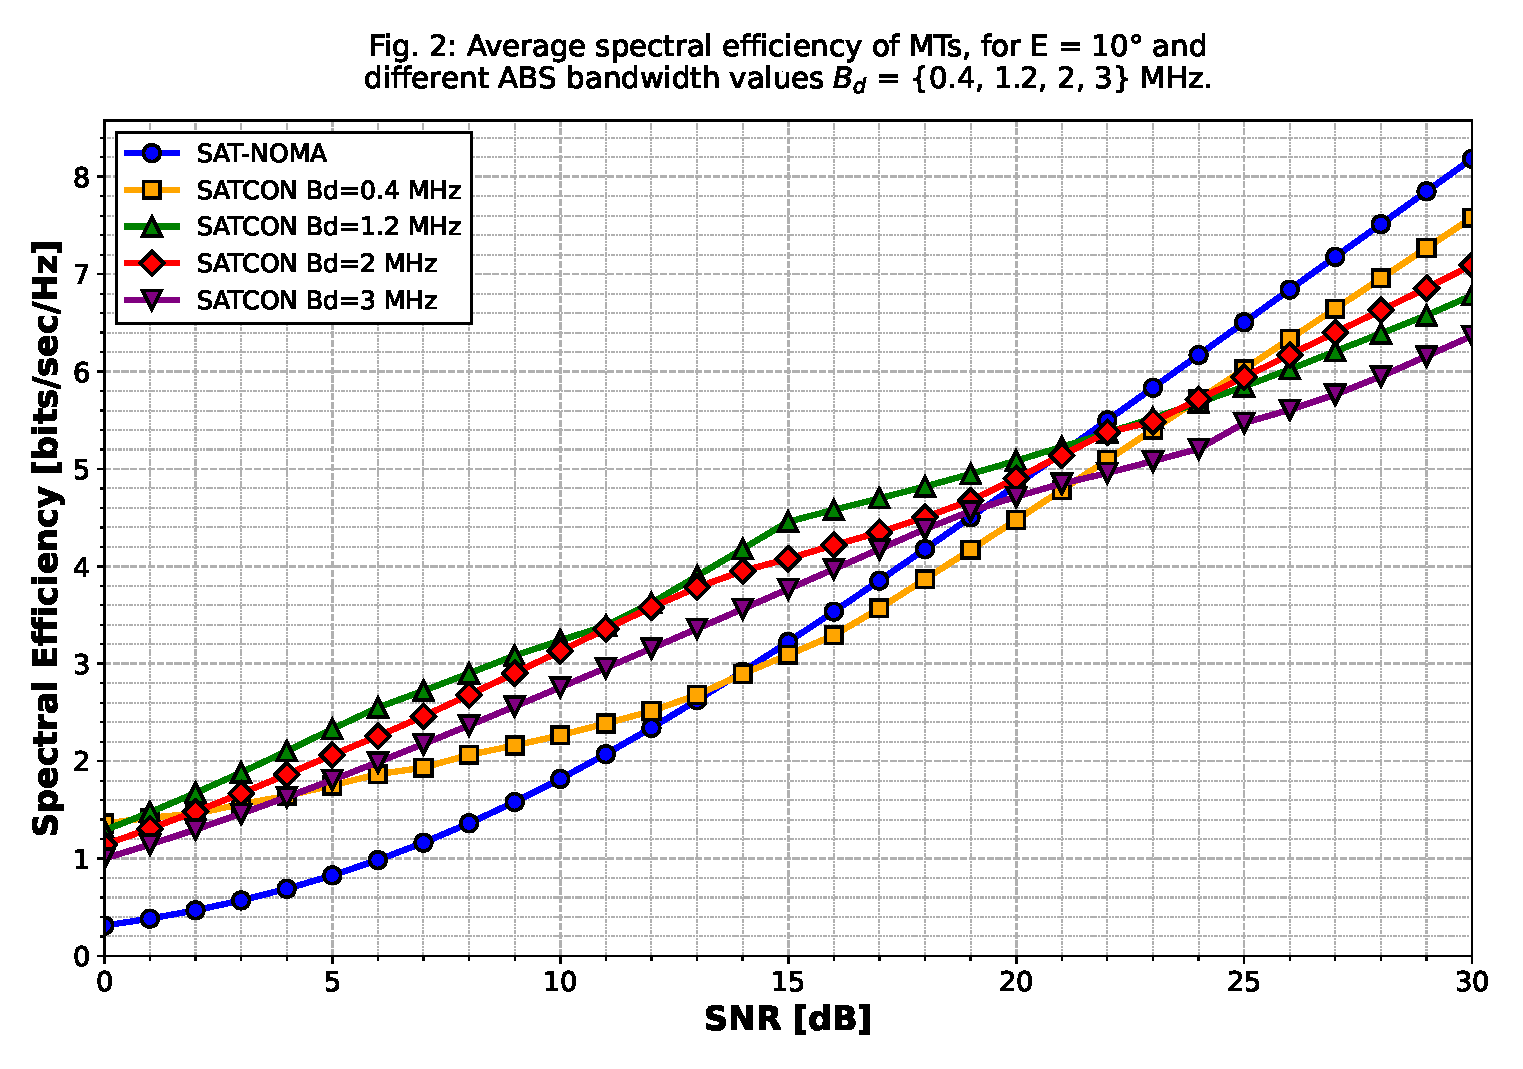
\includegraphics[width=12.5cm]{Definitions/fig2_abs_bandwidth_impact}
\caption{Average spectral efficiency versus SNR for different ABS bandwidth values at a low satellite elevation angle ($E=10^\circ$).}
\label{fig:se_abs_bandwidth}
\end{figure}

Figure~\ref{fig:se_abs_bandwidth} illustrates the average spectral efficiency of mobile terminals as a function of SNR for a low satellite elevation angle of $E=10^\circ$, under different ABS bandwidth configurations. The SAT-NOMA scheme, which relies solely on direct satellite transmission, exhibits the lowest spectral efficiency across the entire SNR range due to severe path loss at low elevation angles.

By contrast, SATCON significantly improves spectral efficiency by leveraging ABS-assisted relaying. When the ABS bandwidth is limited ($B_d=0.4$~MHz), the performance gain over SAT-NOMA remains modest, indicating that the ABS-to-ground link becomes a bottleneck. As $B_d$ increases to $1.2$~MHz, a noticeable improvement is observed, demonstrating that moderate ABS bandwidth is sufficient to effectively support relay-assisted transmission.

Further increasing the ABS bandwidth to $2.0$~MHz and $3.0$~MHz continues to enhance spectral efficiency, although the marginal gain gradually diminishes. This behavior suggests that, beyond a certain point, the end-to-end performance becomes constrained by the satellite-to-ABS link rather than the ABS access link. Overall, Fig.~2 confirms that appropriate ABS bandwidth provisioning is crucial for unlocking the benefits of SATCON, especially under low-elevation satellite scenarios.
\begin{figure}[H]
%\isPreprints{\centering}{} % Only used for preprints
\centering
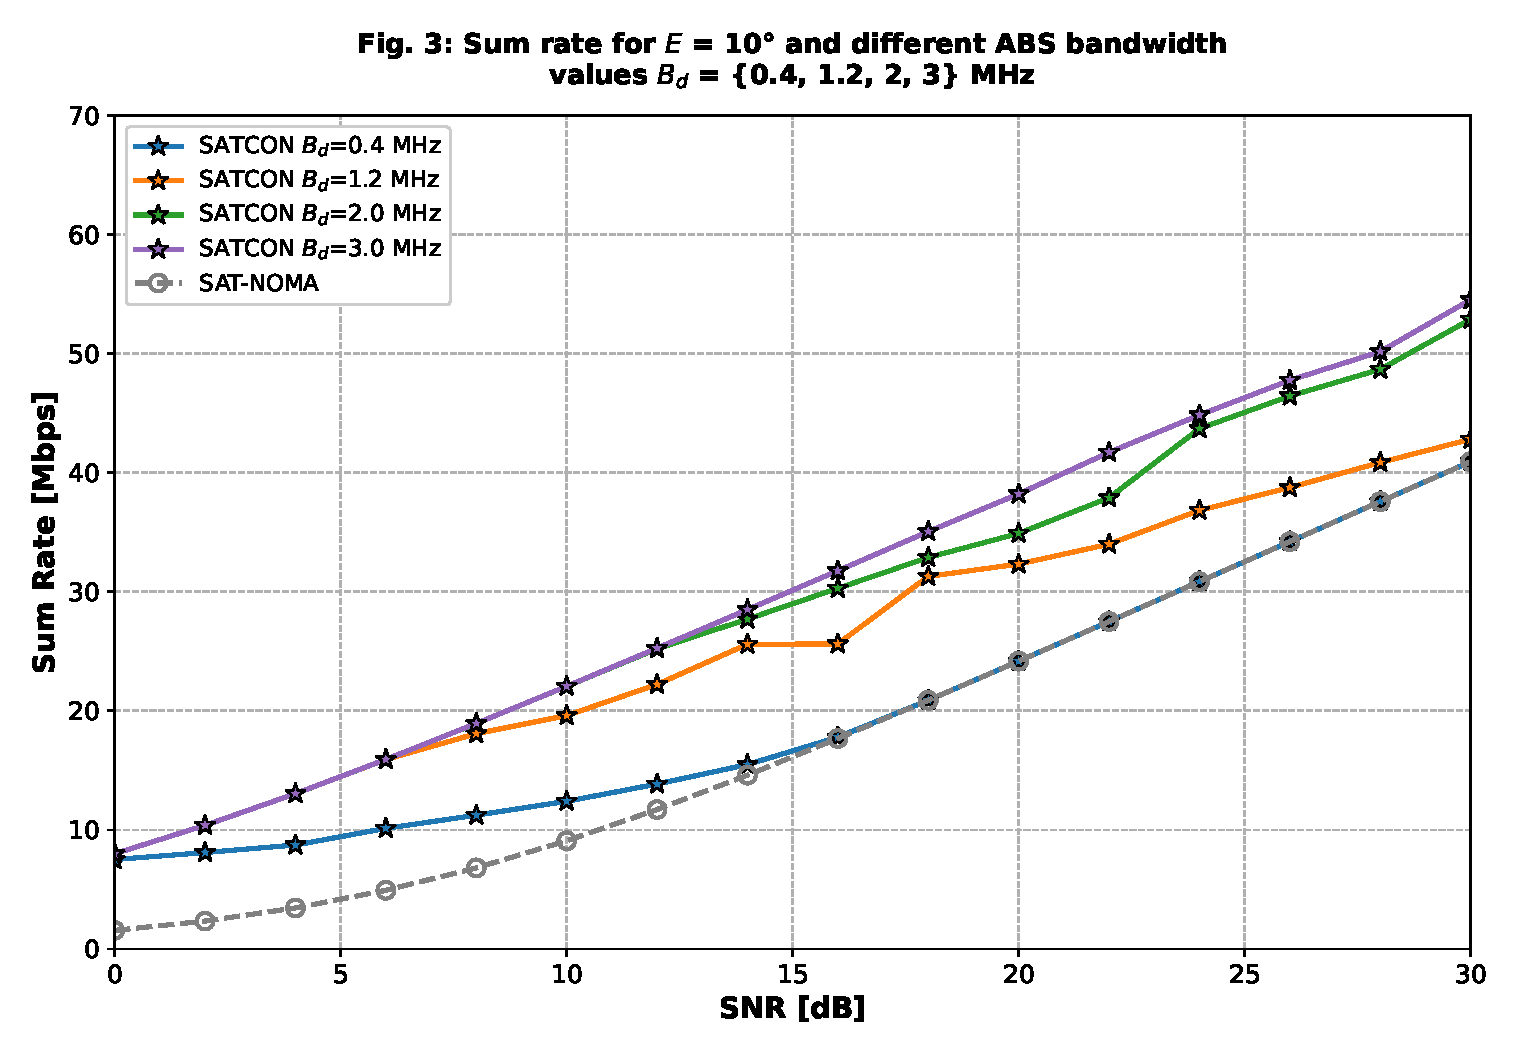
\includegraphics[width=12.5cm]{Definitions/figure3_bandwidth_impact}
\caption{System sum rate versus SNR for different ABS bandwidth values at a low satellite elevation angle ($E=10^\circ$).}
\label{fig:sumrate_abs_bandwidth}
\end{figure}

Figure~\ref{fig:sumrate_abs_bandwidth} depicts the system sum rate as a function of SNR for a low satellite elevation angle of $E=10^\circ$ under different ABS bandwidth configurations. Consistent with the spectral efficiency trends observed in Fig.~2, the proposed SATCON framework achieves a significantly higher sum rate than the SAT-NOMA baseline across the entire SNR range.

When the ABS bandwidth is small ($B_d=0.4$~MHz), SATCON provides only a marginal improvement over SAT-NOMA, indicating that the limited ABS access capacity restricts the effectiveness of relay-assisted transmission. As the ABS bandwidth increases to $1.2$~MHz, a clear performance gain emerges, demonstrating that moderate ABS bandwidth is sufficient to substantially enhance the end-to-end throughput. Further increasing $B_d$ to $2.0$~MHz and $3.0$~MHz leads to additional sum rate improvements, particularly in the medium-to-high SNR regime.

Notably, the growth rate of the sum rate gradually slows down as $B_d$ becomes large, suggesting that the satellite-to-ABS backhaul link increasingly dominates the end-to-end performance. This observation highlights a practical design trade-off: allocating excessive ABS bandwidth yields diminishing returns when the satellite link capacity becomes the primary bottleneck. Overall, Fig.~3 confirms that SATCON can effectively translate spectral efficiency gains into tangible throughput improvements, while also revealing the optimal ABS bandwidth range for cost-efficient deployment.
\begin{figure}[H]
%\isPreprints{\centering}{} % Only used for preprints
\centering
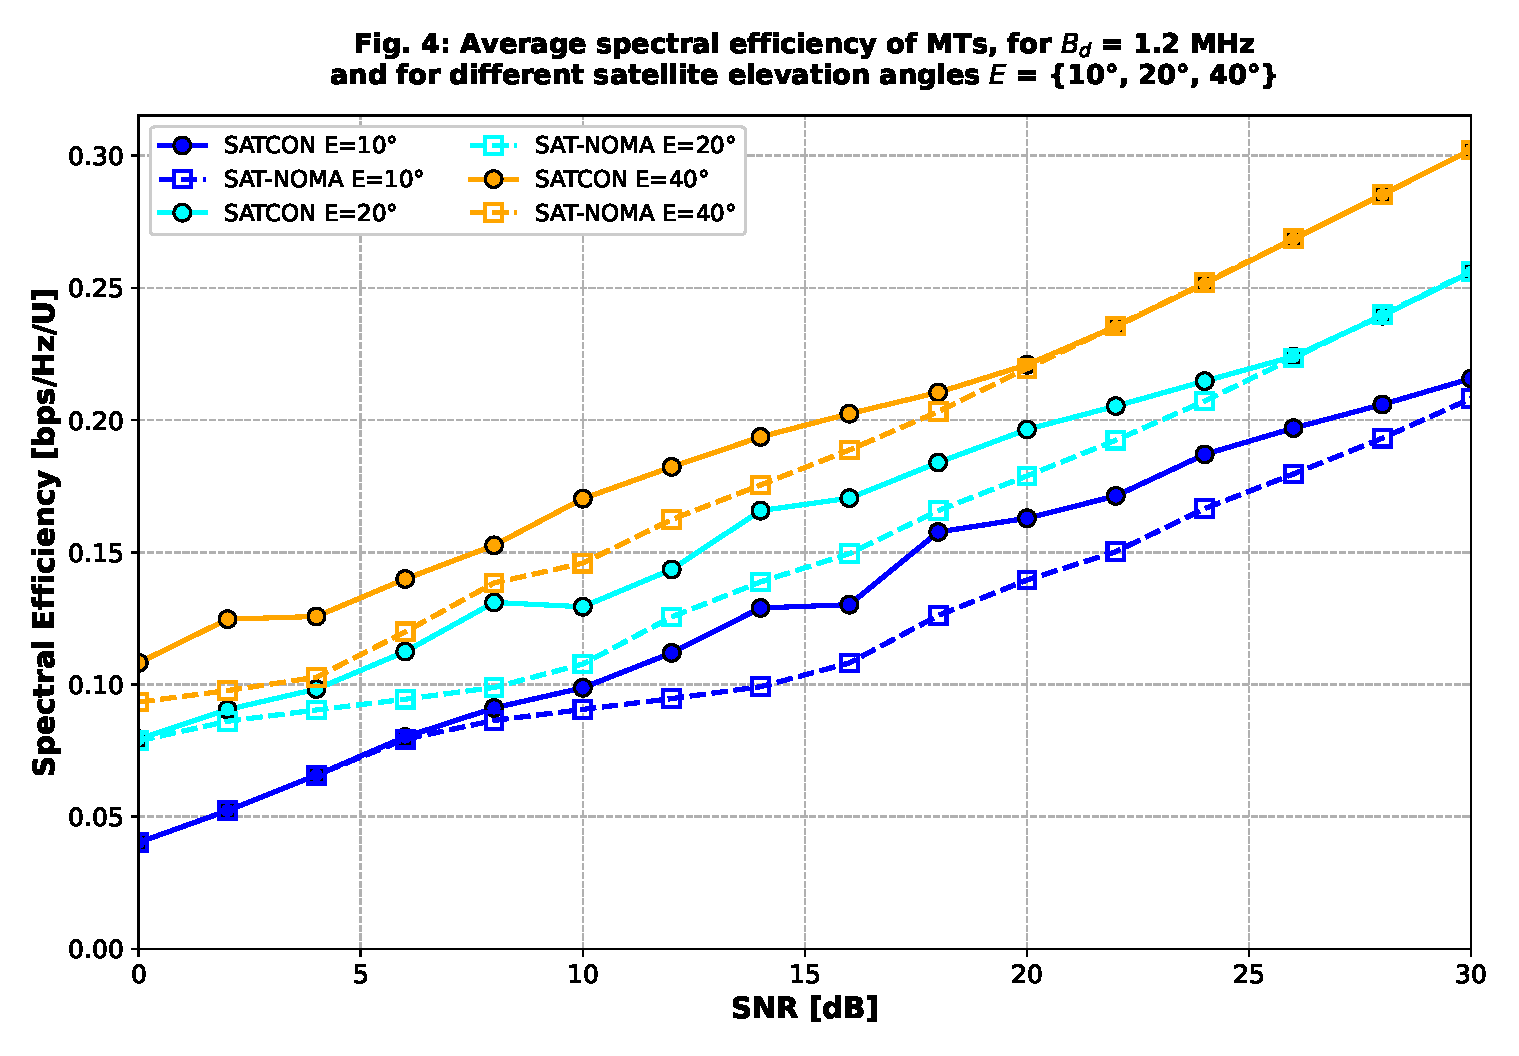
\includegraphics[width=12.5cm]{Definitions/figure4_elevation_impact}
\caption{Average spectral efficiency versus SNR for different satellite elevation angles with a fixed ABS bandwidth of $B_d=1.2$~MHz.}
\label{fig:se_elevation}
\end{figure}

Figure~\ref{fig:se_elevation} shows the average spectral efficiency as a function of SNR for different satellite elevation angles, with the ABS bandwidth fixed at $B_d=1.2$~MHz. The SAT-NOMA baseline and the proposed SATCON framework are compared under identical system settings.

It can be observed that the spectral efficiency of both schemes improves as the elevation angle increases from $10^\circ$ to $40^\circ$, due to the reduced propagation distance and path loss of the satellite links. However, the relative performance gain provided by SATCON strongly depends on the elevation angle. At low elevation ($E=10^\circ$), SATCON achieves a clear and consistent advantage over SAT-NOMA across the entire SNR range, indicating that ABS-assisted relaying is particularly effective in mitigating severe propagation losses.

When the elevation angle increases to $E=20^\circ$, the performance gap between SATCON and SAT-NOMA becomes smaller but remains noticeable, especially in the medium-to-high SNR regime. In contrast, for a high elevation angle of $E=40^\circ$, the two schemes exhibit nearly identical spectral efficiency, suggesting that the direct satellite link already provides near-optimal performance and leaves limited room for ABS-assisted enhancement.

These results demonstrate that the primary benefit of SATCON arises under challenging propagation conditions, such as low-elevation satellite passes, whereas its advantage naturally diminishes in favorable channel scenarios. This behavior confirms that SATCON does not artificially inflate performance but instead adapts its gain to the actual severity of the wireless environment.


\subsection{Figures, Tables and Schemes}

\begin{figure}[H]
%\isPreprints{\centering}{} % Only used for preprints
\centering
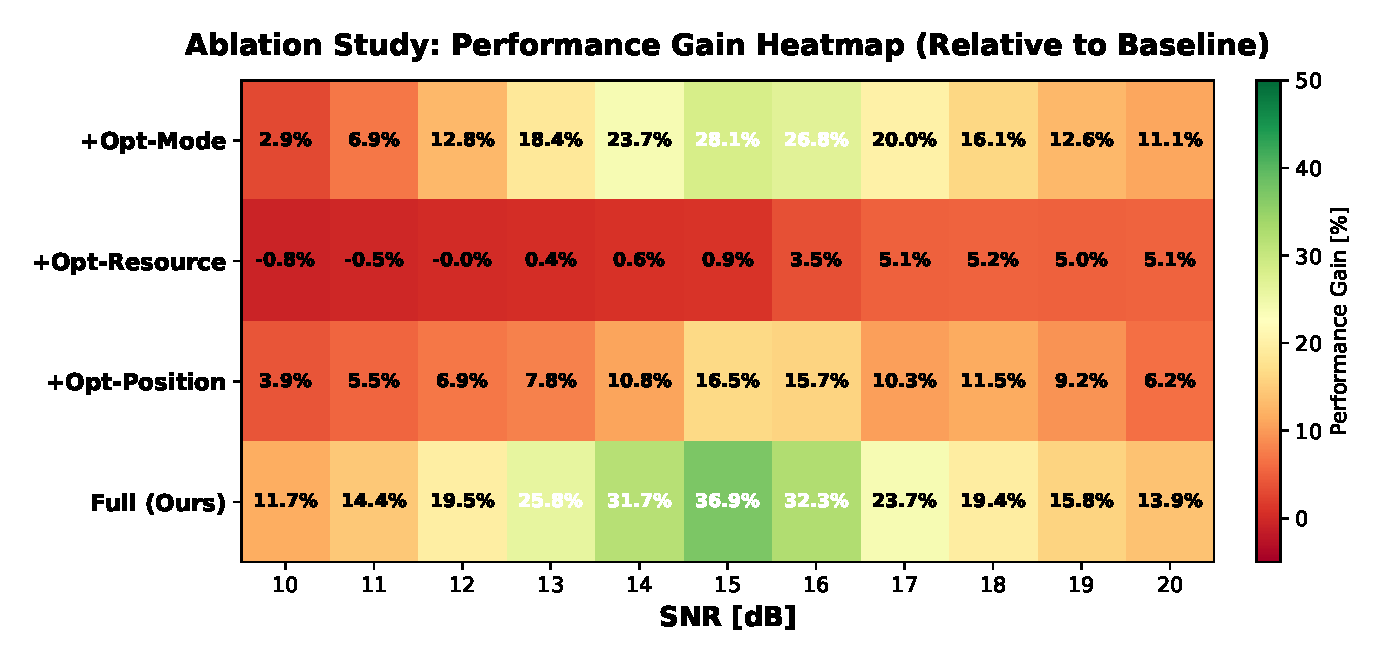
\includegraphics[width=12.5cm]{Definitions/ablation_heatmap_final}
\caption{Ablation study showing the relative performance gain of different optimization components with respect to the baseline scheme under varying SNR conditions.}
\label{fig:ablation_heatmap}
\end{figure}
To quantify the contribution of each optimization component in SATCON, we conduct an ablation study by selectively enabling different modules while keeping all other system parameters unchanged. The baseline scheme corresponds to the heuristic transmission mode selection with uniform bandwidth allocation and k-means-based ABS placement.

Fig.~\ref{fig:ablation_heatmap} illustrates the relative performance gain of different configurations with respect to the baseline under varying SNR conditions. It can be observed that optimizing transmission mode selection alone provides limited performance improvement, especially in the low-SNR regime. Similarly, resource allocation optimization yields only marginal gains when applied in isolation.

In contrast, ABS position optimization contributes a noticeably larger performance gain, indicating that spatial deployment plays a dominant role in improving system throughput. When all three components are jointly optimized, SATCON achieves the highest performance gain across all SNR values, with the maximum improvement exceeding 30\% around $\mathrm{SNR}=15$~dB.

These results demonstrate that no single optimization module is sufficient to fully exploit the system potential. Instead, the performance advantage of SATCON stems from the joint optimization of transmission mode selection, resource allocation, and ABS placement, with position optimization being the most influential component.

\begin{figure}[H]
%\isPreprints{\centering}{} % Only used for preprints
\centering
\includegraphics[width=12.5cm]{Definitions/comparison_baseline_3d}
\caption{Three-dimensional user distribution and ABS placement obtained by the baseline scheme (Heuristic + Uniform + k-means) at $E=10^\circ$ and $\mathrm{SNR}=15$~dB.}
\label{fig:baseline_3d}
\end{figure}

\begin{figure}[H]
%\isPreprints{\centering}{} % Only used for preprints
\centering
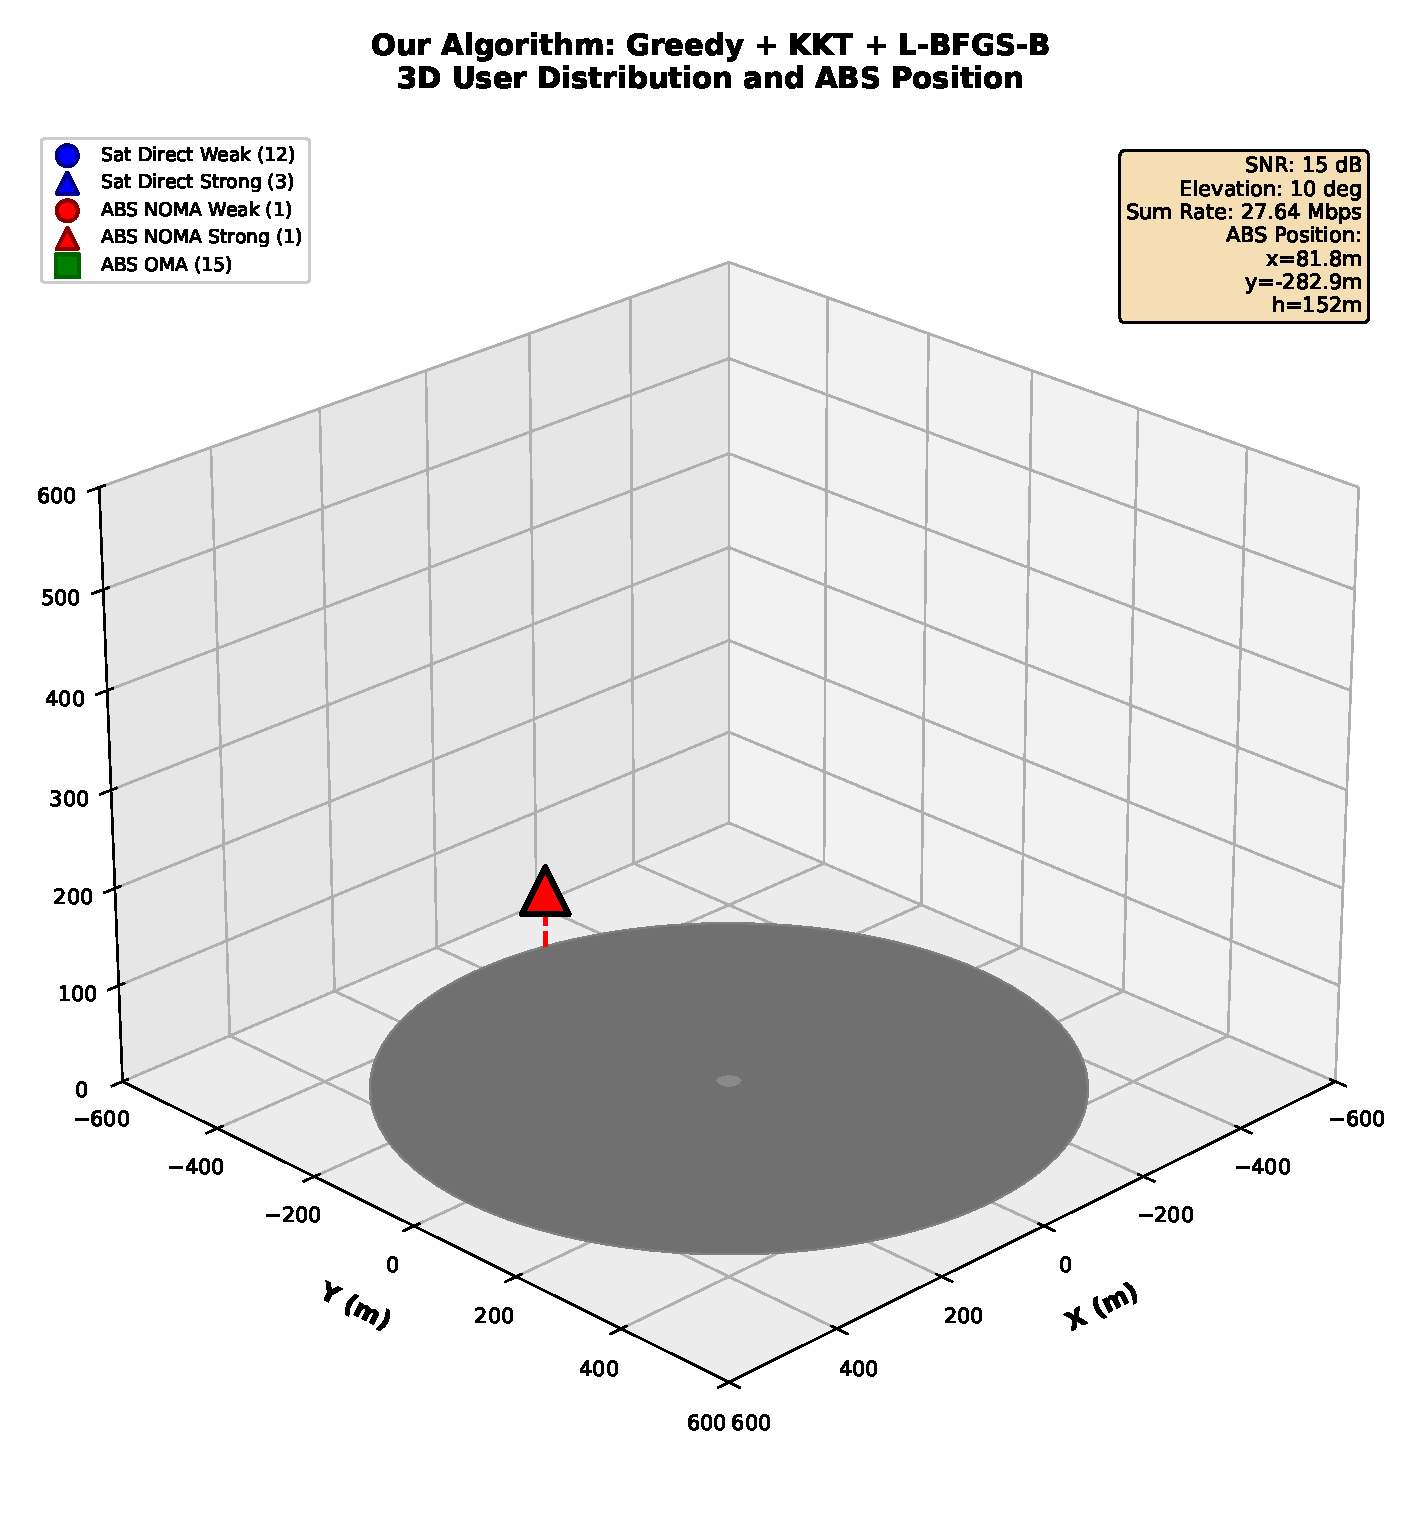
\includegraphics[width=12.5cm]{Definitions/comparison_ours_3d}
\caption{Three-dimensional user distribution and optimized ABS placement obtained by SATCON (Greedy + KKT + L-BFGS-B) under the same system settings as Fig.~\ref{fig:baseline_3d}.}
\label{fig:ours_3d}
\end{figure}

To further illustrate the impact of ABS placement optimization, Fig.~\ref{fig:baseline_3d} and Fig.~\ref{fig:ours_3d} visualize the three-dimensional user distribution and the resulting ABS positions obtained by the baseline scheme and SATCON, respectively.

As shown in Fig.~\ref{fig:baseline_3d}, the baseline method places the ABS near the geometric center of the user distribution, without explicitly considering heterogeneous channel conditions or transmission modes. In contrast, Fig.~\ref{fig:ours_3d} shows that SATCON positions the ABS at a different location and altitude, reflecting a more balanced trade-off between satellite-to-ABS and ABS-to-ground link qualities.

This difference in spatial deployment leads to a significantly higher system sum rate under identical system settings. The visualization confirms that SATCON does not merely improve performance through numerical optimization, but also induces a meaningful structural change in ABS deployment that better adapts to the underlying wireless environment.

\begin{figure}[H]
%\isPreprints{\centering}{} % Only used for preprints
\centering
\includegraphics[width=12.5cm]{Definitions/scalability_analysis}
\caption{Scalability analysis of SATCON and the baseline scheme in terms of average user rate under different numbers of users ($E=10^\circ$, $\mathrm{SNR}=15$~dB, $B_d=1.2$~MHz).}
\label{fig:scalability}
\end{figure}

To evaluate the scalability of the proposed framework, we analyze system performance under different numbers of users while keeping the total bandwidth fixed. Fig.~\ref{fig:scalability} compares the average user rate achieved by SATCON and the baseline scheme for $N=32$, $64$, and $100$ users.

As expected, the average user rate decreases for both schemes as the number of users increases, due to intensified resource sharing. However, SATCON consistently outperforms the baseline across all network sizes, maintaining a nearly constant relative performance gain of approximately 30\%.

This result indicates that the effectiveness of SATCON does not diminish as the network scales. The joint optimization framework adapts to increased user density by dynamically adjusting ABS placement and resource allocation, demonstrating its practical applicability to moderately large-scale satellite–terrestrial integrated networks.


%%%%%%%%%%%%%%%%%%%%%%%%%%%%%%%%%%%%%%%%%%
\section{Discussion}

Authors should discuss the results and how they can be interpreted from the perspective of previous studies and of the working hypotheses. The findings and their implications should be discussed in the broadest context possible. Future research directions may also be highlighted.

%%%%%%%%%%%%%%%%%%%%%%%%%%%%%%%%%%%%%%%%%%
\section{Conclusions}

This section is not mandatory, but can be added to the manuscript if the discussion is unusually long or complex.

%%%%%%%%%%%%%%%%%%%%%%%%%%%%%%%%%%%%%%%%%%
\section{Patents}

This section is not mandatory, but may be added if there are patents resulting from the work reported in this manuscript.

%%%%%%%%%%%%%%%%%%%%%%%%%%%%%%%%%%%%%%%%%%
\vspace{6pt} 

%%%%%%%%%%%%%%%%%%%%%%%%%%%%%%%%%%%%%%%%%%
%% optional
%\supplementary{The following supporting information can be downloaded at:  \linksupplementary{s1}, Figure S1: title; Table S1: title; Video S1: title.}

% Only for journal Methods and Protocols:
% If you wish to submit a video article, please do so with any other supplementary material.
% \supplementary{The following supporting information can be downloaded at: \linksupplementary{s1}, Figure S1: title; Table S1: title; Video S1: title. A supporting video article is available at doi: link.}

% Only used for preprtints:
% \supplementary{The following supporting information can be downloaded at the website of this paper posted on \href{https://www.preprints.org/}{Preprints.org}.}

% Only for journal Hardware:
% If you wish to submit a video article, please do so with any other supplementary material.
% \supplementary{The following supporting information can be downloaded at: \linksupplementary{s1}, Figure S1: title; Table S1: title; Video S1: title.\vspace{6pt}\\
%\begin{tabularx}{\textwidth}{lll}
%\toprule
%\textbf{Name} & \textbf{Type} & \textbf{Description} \\
%\midrule
%S1 & Python script (.py) & Script of python source code used in XX \\
%S2 & Text (.txt) & Script of modelling code used to make Figure X \\
%S3 & Text (.txt) & Raw data from experiment X \\
%S4 & Video (.mp4) & Video demonstrating the hardware in use \\
%... & ... & ... \\
%\bottomrule
%\end{tabularx}
%}

%%%%%%%%%%%%%%%%%%%%%%%%%%%%%%%%%%%%%%%%%%
\authorcontributions{For research articles with several authors, a short paragraph specifying their individual contributions must be provided. The following statements should be used ``Conceptualization, X.X. and Y.Y.; methodology, X.X.; software, X.X.; validation, X.X., Y.Y. and Z.Z.; formal analysis, X.X.; investigation, X.X.; resources, X.X.; data curation, X.X.; writing---original draft preparation, X.X.; writing---review and editing, X.X.; visualization, X.X.; supervision, X.X.; project administration, X.X.; funding acquisition, Y.Y. All authors have read and agreed to the published version of the manuscript.'', please turn to the  \href{http://img.mdpi.org/data/contributor-role-instruction.pdf}{CRediT taxonomy} for the term explanation. Authorship must be limited to those who have contributed substantially to the work~reported.}

\funding{Please add: ``This research received no external funding'' or ``This research was funded by NAME OF FUNDER grant number XXX.'' and  and ``The APC was funded by XXX''. Check carefully that the details given are accurate and use the standard spelling of funding agency names at \url{https://search.crossref.org/funding}, any errors may affect your future funding.}

\institutionalreview{In this section, you should add the Institutional Review Board Statement and approval number, if relevant to your study. You might choose to exclude this statement if the study did not require ethical approval. Please note that the Editorial Office might ask you for further information. Please add “The study was conducted in accordance with the Declaration of Helsinki, and approved by the Institutional Review Board (or Ethics Committee) of NAME OF INSTITUTE (protocol code XXX and date of approval).” for studies involving humans. OR “The animal study protocol was approved by the Institutional Review Board (or Ethics Committee) of NAME OF INSTITUTE (protocol code XXX and date of approval).” for studies involving animals. OR “Ethical review and approval were waived for this study due to REASON (please provide a detailed justification).” OR “Not applicable” for studies not involving humans or animals.}

\informedconsent{Any research article describing a study involving humans should contain this statement. Please add ``Informed consent was obtained from all subjects involved in the study.'' OR ``Patient consent was waived due to REASON (please provide a detailed justification).'' OR ``Not applicable'' for studies not involving humans. You might also choose to exclude this statement if the study did not involve humans.

Written informed consent for publication must be obtained from participating patients who can be identified (including by the patients themselves). Please state ``Written informed consent has been obtained from the patient(s) to publish this paper'' if applicable.}

\dataavailability{We encourage all authors of articles published in MDPI journals to share their research data. In this section, please provide details regarding where data supporting reported results can be found, including links to publicly archived datasets analyzed or generated during the study. Where no new data were created, or where data is unavailable due to privacy or ethical restrictions, a statement is still required. Suggested Data Availability Statements are available in section ``MDPI Research Data Policies'' at \url{https://www.mdpi.com/ethics}.} 

% Only for journal Drones
%\durcstatement{Current research is limited to the [please insert a specific academic field, e.g., XXX], which is beneficial [share benefits and/or primary use] and does not pose a threat to public health or national security. Authors acknowledge the dual-use potential of the research involving xxx and confirm that all necessary precautions have been taken to prevent potential misuse. As an ethical responsibility, authors strictly adhere to relevant national and international laws about DURC. Authors advocate for responsible deployment, ethical considerations, regulatory compliance, and transparent reporting to mitigate misuse risks and foster beneficial outcomes.}

% Only for journal Nursing Reports
%\publicinvolvement{Please describe how the public (patients, consumers, carers) were involved in the research. Consider reporting against the GRIPP2 (Guidance for Reporting Involvement of Patients and the Public) checklist. If the public were not involved in any aspect of the research add: ``No public involvement in any aspect of this research''.}
%
%% Only for journal Nursing Reports
%\guidelinesstandards{Please add a statement indicating which reporting guideline was used when drafting the report. For example, ``This manuscript was drafted against the XXX (the full name of reporting guidelines and citation) for XXX (type of research) research''. A complete list of reporting guidelines can be accessed via the equator network: \url{https://www.equator-network.org/}.}
%
%% Only for journal Nursing Reports
%\useofartificialintelligence{Please describe in detail any and all uses of artificial intelligence (AI) or AI-assisted tools used in the preparation of the manuscript. This may include, but is not limited to, language translation, language editing and grammar, or generating text. Alternatively, please state that “AI or AI-assisted tools were not used in drafting any aspect of this manuscript”.}

\acknowledgments{In this section you can acknowledge any support given which is not covered by the author contribution or funding sections. This may include administrative and technical support, or donations in kind (e.g., materials used for experiments). Where GenAI has been used for purposes such as generating text, data, or graphics, or for study design, data collection, analysis, or interpretation of data, please add “During the preparation of this manuscript/study, the author(s) used [tool name, version information] for the purposes of [description of use]. The authors have reviewed and edited the output and take full responsibility for the content of this publication.”}

\conflictsofinterest{Declare conflicts of interest or state ``The authors declare no conflicts of interest.'' Authors must identify and declare any personal circumstances or interest that may be perceived as inappropriately influencing the representation or interpretation of reported research results. Any role of the funders in the design of the study; in the collection, analyses or interpretation of data; in the writing of the manuscript; or in the decision to publish the results must be declared in this section. If there is no role, please state ``The funders had no role in the design of the study; in the collection, analyses, or interpretation of data; in the writing of the manuscript; or in the decision to publish the results''.} 

%%%%%%%%%%%%%%%%%%%%%%%%%%%%%%%%%%%%%%%%%%
%% Optional

%% Only for journal Encyclopedia
%\entrylink{The Link to this entry published on the encyclopedia platform.}

\abbreviations{Abbreviations}{
The following abbreviations are used in this manuscript:
\\

\noindent 
\begin{tabular}{@{}ll}
MDPI & Multidisciplinary Digital Publishing Institute\\
DOAJ & Directory of open access journals\\
TLA & Three letter acronym\\
LD & Linear dichroism
\end{tabular}
}

%%%%%%%%%%%%%%%%%%%%%%%%%%%%%%%%%%%%%%%%%%
%% Optional
\appendixtitles{no} % Leave argument "no" if all appendix headings stay EMPTY (then no dot is printed after "Appendix A"). If the appendix sections contain a heading then change the argument to "yes".
\appendixstart
\appendix
\section[\appendixname~\thesection]{}
\subsection[\appendixname~\thesubsection]{}
The appendix is an optional section that can contain details and data supplemental to the main text---for example, explanations of experimental details that would disrupt the flow of the main text but nonetheless remain crucial to understanding and reproducing the research shown; figures of replicates for experiments of which representative data are shown in the main text can be added here if brief, or as Supplementary Data. Mathematical proofs of results not central to the paper can be added as an appendix.

\begin{table}[H] 
\caption{This is a table caption.\label{tab5}}
%\newcolumntype{C}{>{\centering\arraybackslash}X}
\begin{tabularx}{\textwidth}{CCC}
\toprule
\textbf{Title 1}	& \textbf{Title 2}	& \textbf{Title 3}\\
\midrule
Entry 1		& Data			& Data\\
Entry 2		& Data			& Data\\
\bottomrule
\end{tabularx}
\end{table}

\section[\appendixname~\thesection]{}
All appendix sections must be cited in the main text. In the appendices, Figures, Tables, etc. should be labeled, starting with ``A''---e.g., Figure A1, Figure A2, etc.

%%%%%%%%%%%%%%%%%%%%%%%%%%%%%%%%%%%%%%%%%%
%\isPreprints{} % If the paper is ``preprints'', please uncomment this parenthesis.
%\printendnotes[custom] % Un-comment to print a list of endnotes

\reftitle{References}

% Please provide the correct journal abbreviation (e.g. according to the “List of Title Word Abbreviations” http://www.issn.org/services/online-services/access-to-the-ltwa/).
% Citations and References in Supplementary files are permitted provided that they also appear in the reference list here. 

%=====================================
% References, variant A: external bibliography
%=====================================
% \bibliography{your_external_BibTeX_file}

%=====================================
% References, variant B: internal bibliography
%=====================================

% ACS format
\begin{thebibliography}{999}
% Reference 1
\bibitem{ref-journal}
Author~1, T. The title of the cited article. {\em Journal Abbreviation} {\bf 2008}, {\em 10}, 142--149.
% Reference 2
\bibitem{ref-book1}
Author~2, L. The title of the cited contribution. In {\em The Book Title}; Editor 1, F., Editor 2, A., Eds.; Publishing House: City, Country, 2007; pp. 32--58.
% Reference 3
\bibitem{ref-book2}
Author 1, A.; Author 2, B. \textit{Book Title}, 3rd ed.; Publisher: Publisher Location, Country, 2008; pp. 154--196.
% Reference 4
\bibitem{ref-unpublish}
Author 1, A.B.; Author 2, C. Title of Unpublished Work. \textit{Abbreviated Journal Name} year, \textit{phrase indicating stage of publication (submitted; accepted; in press)}.
% Reference 5
\bibitem{ref-url}
Title of Site. Available online: URL (accessed on Day Month Year).
% Reference 6
\bibitem{ref-proceeding}
Author 1, A.B.; Author 2, C.D.; Author 3, E.F. Title of presentation. In Proceedings of the Name of the Conference, Location of Conference, Country, Date of Conference (Day Month Year); Abstract Number (optional), Pagination (optional).
% Reference 7
\bibitem{ref-thesis}
Author 1, A.B. Title of Thesis. Level of Thesis, Degree-Granting University, Location of University, Date of Completion.
% Reference 8
\bibitem{al2014modeling}
Al-Hourani, A.; Kandeepan, S.; Lardner, S.Optimal LAP Altitude for Maximum Coverage.{\em IEEE Wireless Commun. Lett.} {\bf 2014}, {\em 3}, 569--572.
% Reference 9
\bibitem{zhu2018optimal}
Zhu, L.; Zhang, J.; Xiao, Z.; Cao, X.; Wu, D. O.
Optimal user pairing for downlink non-orthogonal multiple access (NOMA).
{\em IEEE Wireless Commun. Lett.} {\bf 2018}, {\em 8}, 328--331.

\end{thebibliography}

% If authors have biography, please use the format below
%\section*{Short Biography of Authors}
%\bio
%{\raisebox{-0.35cm}{\includegraphics[width=3.5cm,height=5.3cm,clip,keepaspectratio]{Definitions/author1.pdf}}}
%{\textbf{Firstname Lastname} Biography of first author}
%
%\bio
%{\raisebox{-0.35cm}{\includegraphics[width=3.5cm,height=5.3cm,clip,keepaspectratio]{Definitions/author2.jpg}}}
%{\textbf{Firstname Lastname} Biography of second author}

% For the MDPI journals use author-date citation, please follow the formatting guidelines on http://www.mdpi.com/authors/references
% To cite two works by the same author: \citeauthor{ref-journal-1a} (\citeyear{ref-journal-1a}, \citeyear{ref-journal-1b}). This produces: Whittaker (1967, 1975)
% To cite two works by the same author with specific pages: \citeauthor{ref-journal-3a} (\citeyear{ref-journal-3a}, p. 328; \citeyear{ref-journal-3b}, p.475). This produces: Wong (1999, p. 328; 2000, p. 475)

%%%%%%%%%%%%%%%%%%%%%%%%%%%%%%%%%%%%%%%%%%
%% for journal Sci
%\reviewreports{\\
%Reviewer 1 comments and authors’ response\\
%Reviewer 2 comments and authors’ response\\
%Reviewer 3 comments and authors’ response
%}
%%%%%%%%%%%%%%%%%%%%%%%%%%%%%%%%%%%%%%%%%%
\PublishersNote{}
%\isPreprints{} % If the paper is ``preprints'', please uncomment this parenthesis.
\end{document}

